% Created by tikzDevice version 0.12
% !TEX encoding = UTF-8 Unicode
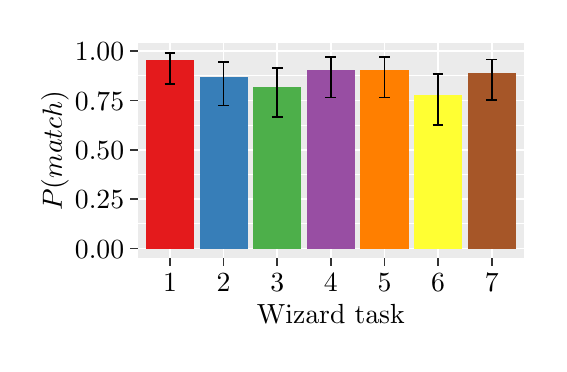
\begin{tikzpicture}[x=1pt,y=1pt]
\definecolor{fillColor}{RGB}{255,255,255}
\path[use as bounding box,fill=fillColor,fill opacity=0.00] (0,0) rectangle (184.80,114.21);
\begin{scope}
\path[clip] (  0.00,  0.00) rectangle (184.80,114.21);
\definecolor{drawColor}{RGB}{255,255,255}
\definecolor{fillColor}{RGB}{255,255,255}

\path[draw=drawColor,line width= 0.6pt,line join=round,line cap=round,fill=fillColor] (  0.00,  0.00) rectangle (184.80,114.21);
\end{scope}
\begin{scope}
\path[clip] ( 39.80, 30.86) rectangle (179.30,108.71);
\definecolor{fillColor}{gray}{0.92}

\path[fill=fillColor] ( 39.80, 30.86) rectangle (179.30,108.71);
\definecolor{drawColor}{RGB}{255,255,255}

\path[draw=drawColor,line width= 0.3pt,line join=round] ( 39.80, 43.32) --
	(179.30, 43.32);

\path[draw=drawColor,line width= 0.3pt,line join=round] ( 39.80, 61.15) --
	(179.30, 61.15);

\path[draw=drawColor,line width= 0.3pt,line join=round] ( 39.80, 78.98) --
	(179.30, 78.98);

\path[draw=drawColor,line width= 0.3pt,line join=round] ( 39.80, 96.82) --
	(179.30, 96.82);

\path[draw=drawColor,line width= 0.6pt,line join=round] ( 39.80, 34.40) --
	(179.30, 34.40);

\path[draw=drawColor,line width= 0.6pt,line join=round] ( 39.80, 52.23) --
	(179.30, 52.23);

\path[draw=drawColor,line width= 0.6pt,line join=round] ( 39.80, 70.07) --
	(179.30, 70.07);

\path[draw=drawColor,line width= 0.6pt,line join=round] ( 39.80, 87.90) --
	(179.30, 87.90);

\path[draw=drawColor,line width= 0.6pt,line join=round] ( 39.80,105.73) --
	(179.30,105.73);

\path[draw=drawColor,line width= 0.6pt,line join=round] ( 51.43, 30.86) --
	( 51.43,108.71);

\path[draw=drawColor,line width= 0.6pt,line join=round] ( 70.80, 30.86) --
	( 70.80,108.71);

\path[draw=drawColor,line width= 0.6pt,line join=round] ( 90.18, 30.86) --
	( 90.18,108.71);

\path[draw=drawColor,line width= 0.6pt,line join=round] (109.55, 30.86) --
	(109.55,108.71);

\path[draw=drawColor,line width= 0.6pt,line join=round] (128.93, 30.86) --
	(128.93,108.71);

\path[draw=drawColor,line width= 0.6pt,line join=round] (148.30, 30.86) --
	(148.30,108.71);

\path[draw=drawColor,line width= 0.6pt,line join=round] (167.68, 30.86) --
	(167.68,108.71);
\definecolor{fillColor}{RGB}{228,26,28}

\path[fill=fillColor] ( 42.71, 34.40) rectangle ( 60.15,102.49);
\definecolor{fillColor}{RGB}{55,126,184}

\path[fill=fillColor] ( 62.09, 34.40) rectangle ( 79.52, 96.22);
\definecolor{fillColor}{RGB}{77,175,74}

\path[fill=fillColor] ( 81.46, 34.40) rectangle ( 98.90, 92.76);
\definecolor{fillColor}{RGB}{152,78,163}

\path[fill=fillColor] (100.83, 34.40) rectangle (118.27, 98.94);
\definecolor{fillColor}{RGB}{255,127,0}

\path[fill=fillColor] (120.21, 34.40) rectangle (137.65, 98.94);
\definecolor{fillColor}{RGB}{255,255,51}

\path[fill=fillColor] (139.58, 34.40) rectangle (157.02, 89.88);
\definecolor{fillColor}{RGB}{166,86,40}

\path[fill=fillColor] (158.96, 34.40) rectangle (176.39, 97.81);
\definecolor{drawColor}{RGB}{0,0,0}

\path[draw=drawColor,line width= 0.6pt,line join=round] ( 49.49,105.17) --
	( 53.37,105.17);

\path[draw=drawColor,line width= 0.6pt,line join=round] ( 51.43,105.17) --
	( 51.43, 93.82);

\path[draw=drawColor,line width= 0.6pt,line join=round] ( 49.49, 93.82) --
	( 53.37, 93.82);

\path[draw=drawColor,line width= 0.6pt,line join=round] ( 68.87,101.78) --
	( 72.74,101.78);

\path[draw=drawColor,line width= 0.6pt,line join=round] ( 70.80,101.78) --
	( 70.80, 86.12);

\path[draw=drawColor,line width= 0.6pt,line join=round] ( 68.87, 86.12) --
	( 72.74, 86.12);

\path[draw=drawColor,line width= 0.6pt,line join=round] ( 88.24, 99.52) --
	( 92.12, 99.52);

\path[draw=drawColor,line width= 0.6pt,line join=round] ( 90.18, 99.52) --
	( 90.18, 82.02);

\path[draw=drawColor,line width= 0.6pt,line join=round] ( 88.24, 82.02) --
	( 92.12, 82.02);

\path[draw=drawColor,line width= 0.6pt,line join=round] (107.61,103.52) --
	(111.49,103.52);

\path[draw=drawColor,line width= 0.6pt,line join=round] (109.55,103.52) --
	(109.55, 88.94);

\path[draw=drawColor,line width= 0.6pt,line join=round] (107.61, 88.94) --
	(111.49, 88.94);

\path[draw=drawColor,line width= 0.6pt,line join=round] (126.99,103.52) --
	(130.86,103.52);

\path[draw=drawColor,line width= 0.6pt,line join=round] (128.93,103.52) --
	(128.93, 88.94);

\path[draw=drawColor,line width= 0.6pt,line join=round] (126.99, 88.94) --
	(130.86, 88.94);

\path[draw=drawColor,line width= 0.6pt,line join=round] (146.36, 97.38) --
	(150.24, 97.38);

\path[draw=drawColor,line width= 0.6pt,line join=round] (148.30, 97.38) --
	(148.30, 79.00);

\path[draw=drawColor,line width= 0.6pt,line join=round] (146.36, 79.00) --
	(150.24, 79.00);

\path[draw=drawColor,line width= 0.6pt,line join=round] (165.74,102.76) --
	(169.61,102.76);

\path[draw=drawColor,line width= 0.6pt,line join=round] (167.68,102.76) --
	(167.68, 88.01);

\path[draw=drawColor,line width= 0.6pt,line join=round] (165.74, 88.01) --
	(169.61, 88.01);
\end{scope}
\begin{scope}
\path[clip] (  0.00,  0.00) rectangle (184.80,114.21);
\definecolor{drawColor}{RGB}{0,0,0}

\node[text=drawColor,anchor=base east,inner sep=0pt, outer sep=0pt, scale=  1.00] at ( 34.85, 30.96) {0.00};

\node[text=drawColor,anchor=base east,inner sep=0pt, outer sep=0pt, scale=  1.00] at ( 34.85, 48.79) {0.25};

\node[text=drawColor,anchor=base east,inner sep=0pt, outer sep=0pt, scale=  1.00] at ( 34.85, 66.62) {0.50};

\node[text=drawColor,anchor=base east,inner sep=0pt, outer sep=0pt, scale=  1.00] at ( 34.85, 84.46) {0.75};

\node[text=drawColor,anchor=base east,inner sep=0pt, outer sep=0pt, scale=  1.00] at ( 34.85,102.29) {1.00};
\end{scope}
\begin{scope}
\path[clip] (  0.00,  0.00) rectangle (184.80,114.21);
\definecolor{drawColor}{gray}{0.20}

\path[draw=drawColor,line width= 0.6pt,line join=round] ( 37.05, 34.40) --
	( 39.80, 34.40);

\path[draw=drawColor,line width= 0.6pt,line join=round] ( 37.05, 52.23) --
	( 39.80, 52.23);

\path[draw=drawColor,line width= 0.6pt,line join=round] ( 37.05, 70.07) --
	( 39.80, 70.07);

\path[draw=drawColor,line width= 0.6pt,line join=round] ( 37.05, 87.90) --
	( 39.80, 87.90);

\path[draw=drawColor,line width= 0.6pt,line join=round] ( 37.05,105.73) --
	( 39.80,105.73);
\end{scope}
\begin{scope}
\path[clip] (  0.00,  0.00) rectangle (184.80,114.21);
\definecolor{drawColor}{gray}{0.20}

\path[draw=drawColor,line width= 0.6pt,line join=round] ( 51.43, 28.11) --
	( 51.43, 30.86);

\path[draw=drawColor,line width= 0.6pt,line join=round] ( 70.80, 28.11) --
	( 70.80, 30.86);

\path[draw=drawColor,line width= 0.6pt,line join=round] ( 90.18, 28.11) --
	( 90.18, 30.86);

\path[draw=drawColor,line width= 0.6pt,line join=round] (109.55, 28.11) --
	(109.55, 30.86);

\path[draw=drawColor,line width= 0.6pt,line join=round] (128.93, 28.11) --
	(128.93, 30.86);

\path[draw=drawColor,line width= 0.6pt,line join=round] (148.30, 28.11) --
	(148.30, 30.86);

\path[draw=drawColor,line width= 0.6pt,line join=round] (167.68, 28.11) --
	(167.68, 30.86);
\end{scope}
\begin{scope}
\path[clip] (  0.00,  0.00) rectangle (184.80,114.21);
\definecolor{drawColor}{RGB}{0,0,0}

\node[text=drawColor,anchor=base,inner sep=0pt, outer sep=0pt, scale=  1.00] at ( 51.43, 19.03) {1};

\node[text=drawColor,anchor=base,inner sep=0pt, outer sep=0pt, scale=  1.00] at ( 70.80, 19.03) {2};

\node[text=drawColor,anchor=base,inner sep=0pt, outer sep=0pt, scale=  1.00] at ( 90.18, 19.03) {3};

\node[text=drawColor,anchor=base,inner sep=0pt, outer sep=0pt, scale=  1.00] at (109.55, 19.03) {4};

\node[text=drawColor,anchor=base,inner sep=0pt, outer sep=0pt, scale=  1.00] at (128.93, 19.03) {5};

\node[text=drawColor,anchor=base,inner sep=0pt, outer sep=0pt, scale=  1.00] at (148.30, 19.03) {6};

\node[text=drawColor,anchor=base,inner sep=0pt, outer sep=0pt, scale=  1.00] at (167.68, 19.03) {7};
\end{scope}
\begin{scope}
\path[clip] (  0.00,  0.00) rectangle (184.80,114.21);
\definecolor{drawColor}{RGB}{0,0,0}

\node[text=drawColor,anchor=base,inner sep=0pt, outer sep=0pt, scale=  1.00] at (109.55,  7.44) {Wizard task};
\end{scope}
\begin{scope}
\path[clip] (  0.00,  0.00) rectangle (184.80,114.21);
\definecolor{drawColor}{RGB}{0,0,0}

\node[text=drawColor,rotate= 90.00,anchor=base,inner sep=0pt, outer sep=0pt, scale=  1.00] at ( 12.39, 69.78) {\(P(match)\)};
\end{scope}
\end{tikzpicture}
